\subsection{Statistique descriptive en 2D}


\subsubsection{Covariance}

\begin{center}
	\begin{tabular}{ccc}
		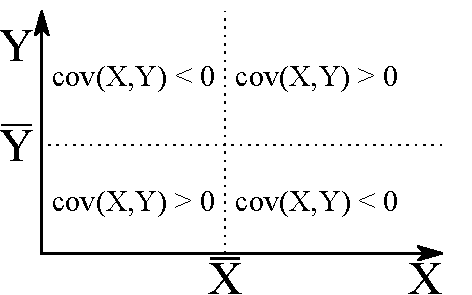
\includegraphics[width=0.3\textwidth]{images/covariance-all.pdf}&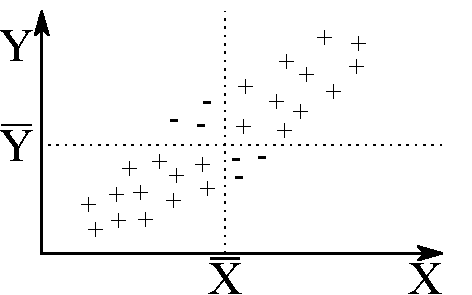
\includegraphics[width=0.3\textwidth]{images/covariance-positive.pdf}&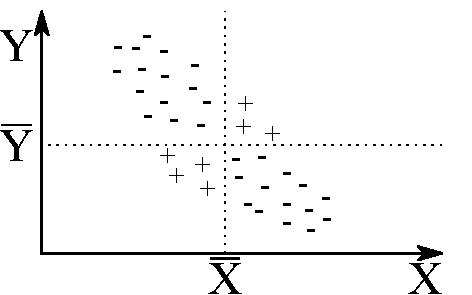
\includegraphics[width=0.3\textwidth]{images/covariance-negative.pdf}\\
		Allure générale&$m_{11}>0$&$m_{11}<0$
	\end{tabular}
\end{center}





\paragraph{La covariance $|m_{11}| \leq s_1s_2$}

La covariance est le moment d'ordre (1,1):

$$m_{11}=\frac{1}{n} \sum_{i=1}^{p} \sum_{j=1}^{q} n_{ij} (x_i-\bar{x})(y_j-\bar{y})$$

\begin{align*}
	0 &\leq \frac{1}{n} \sum_{i=1}^{p} \sum_{j=1}^{q} n_{ij} \underbrace{ ( u (x_i-\bar{x})+(y_j-\bar{y}))^2 }_\text{$^2$ car toujours $\geq 0$} \\
	  &\leq \frac{1}{n} \sum_{i=1}^{p} \sum_{j=1}^{q} n_{ij} (u^2(x_i-\bar{x})^2 + 2u(x_i-\bar{x})(y_j-\bar{y})+(y_j-\bar{y})^2)\\
	  &\leq u^2s_1^2+2u\ m_{11}+s_2^2
\end{align*}

Équation du second degré, on calcule son $\Delta$ :
\begin{align*}
	\Delta &\leq 0\\
	(2 m_{11})^4 - 4 s_1^2 s_2^2 &\leq 0\\
	m_{11}^2 - s_1^2 s_2^2 &\leq 0\\
	m_{11}^2 &\leq s_1^2 s_2^2
\end{align*}
$$\boxed{|m_{11}| \leq s_1 s_2}$$




\paragraph{La covariance maximale $|m_{11}| = s_1s_2$}

La valeur absolue de la covariance est maximale si elle vaut $|m_{11}| = s_1s_2$.

Si les points observés se trouvent sur une droite non parallèle aux axes $ax+by+c=0$, on a $ax_i+by_i+c=0$.

On multiplie par $\frac{n_{ij}}{n}$ et on somme sur $ij$.

\begin{align*}
0  &= \sum_{i=1}^{p} \sum_{j=1}^{q} \frac{n_{ij}}{n}(ax_i+by_j+c) \\
   &= a \frac{1}{n} \sum_{i=1}^{p} \sum_{j=1}^{q}n_{ij}x_i + b \frac{1}{n} \sum_{i=1}^{p} \sum_{j=1}^{q}n_{ij}y_j + c \frac{1}{n} \sum_{i=1}^{p} \sum_{j=1}^{q}n_{ij}\\
   &= a\bar{x}+b\bar{y}+c\\
\intertext{On soustrait $ax_i+by_j+c=0$ par $a\bar{x}+b\bar{y}+c = 0$.}
   &= a(x_i-\bar{x})+b(y_j+\bar{y})\\
\intertext{On utilise $u_0=\frac{a}{b}$}
   &= u_0b(x_i-\bar{x})+b\frac{a}{u_0}(y_j-\bar{y})\\
   &= u_0(x_i-\bar{x})+(y_j-\bar{y})
\end{align*}

L'équation a la même forme que $\alpha$, du coup...
\begin{align*}
	0        &= \Delta\\
	         &= m_{11}^2-s_1^2s_2^2\\
	m_{11}^2 &= s_1^2s_2^2
\end{align*}
$$\boxed{|m_{11}| = s_1s_2}$$









\subsubsection{Le coefficient de corrélation}
$$\boxed{r=\frac{m_{11}}{s_1s_2}}$$
\paragraph{Propriétés}
\begin{enumerate}
	\item $r$ sans dimensions ;
	\item $r' = r$ ;
	\item $-1 \leq r \leq 1$ ;
	\item $|r| = 1$ ssi les points observés se trouvent sur une droite non parallèle aux axes.
\end{enumerate}
\paragraph{Représentation de la droite de régression en fonction du coefficient de corrélation}
\begin{center}
	\begin{tabular}{ccc}
		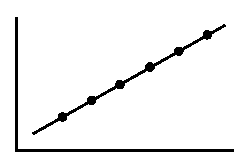
\includegraphics[width=0.2\textwidth]{images/coefficient-correlation1.pdf}&
		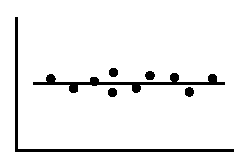
\includegraphics[width=0.2\textwidth]{images/coefficient-correlation0.pdf}&
		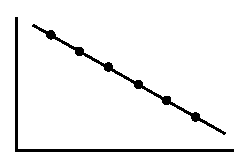
\includegraphics[width=0.2\textwidth]{images/coefficient-correlation-1.pdf}\\
		$r=1$&$r=0$&$r=-1$\\
	\end{tabular}
\end{center}
\begin{itemize}
	\item si $|r| = 1$, il y a une relation fonctionnelle linéaire entre X et Y ;
	\item si $r = 0$, Y est indépendante de X: la covariance est nulle et la droite de régression est horizontale ;
	\item la liaison entre X et Y est d’autant plus intime que |r| est voisin de 1, et d’autant plus faible que |r| est voisin de 0.
\end{itemize}








\newpage
\subsubsection{Les droites de régression}

\begin{center}
	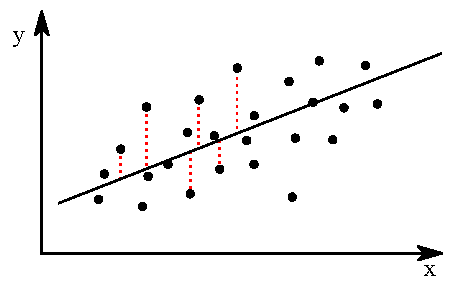
\includegraphics[width=0.3\textwidth]{images/droite_de_regression.pdf}
\end{center}
La droite de régression de y en x est la droite qui minimise la somme des carrés des écarts des points observés à cette droite, les écarts étant pris parall`element à l'axe y. C'est donc la droite d'équation $y = ax+b$ qui minimise la quantité.
$$\boxed{g(a,b) = \sum_{i=1}^{p} \sum_{j=1}^{q} n_{ij} (y_j - a\ x_i - b)^2}$$
Dérivée par rapport à $a$ :
\begin{center}
	$\begin{array}{CCL}
		                & 0 &= \left.g(a,b)\right|_a\\
		\Leftrightarrow & 0 &= \sum_{i=1}^{p} \sum_{j=1}^{q} n_{ij}\ 2(y_j - a\ x_i-b)(-x_i)\\
		\Leftrightarrow & 0 &= \sum_{i=1}^{p} \sum_{j=1}^{q} -2n_{ij}\ x_i(y_j - a\ x_i - b)\\
		\Leftrightarrow & 0 &= \sum_{i=1}^{p} \sum_{j=1}^{q} n_{ij}\ x_i(-y_j + a\ x_i + b)\\
		\Leftrightarrow & 0 &= \sum_{i=1}^{p} \sum_{j=1}^{q} -n_{ij}\ x_i\ y_j + \sum_{i=1}^{p} \sum_{j=1}^{q} n_{ij}\ a\ x_i^2 + \sum_{i=1}^{p} \sum_{j=1}^{q} n_{ij}\ b\ x_i\\
		\Leftrightarrow & 0 &= -1 \sum_{i=1}^{p} \sum_{j=1}^{q} n_{ij}\ x_i\ y_j + a \sum_{i=1}^{p} \sum_{j=1}^{q} n_{ij}\ x_i^2 + b \sum_{i=1}^{p} \sum_{j=1}^{q} n_{ij}\ x_i\\
		\Leftrightarrow &\sum_{i=1}^{p} \sum_{j=1}^{q} n_{ij}\ x_i\ y_j  &= \underbrace{a \sum_{i=1}^{p} \sum_{j=1}^{q} n_{ij}\ x_i^2 + b \sum_{i=1}^{p} \sum_{j=1}^{q} n_{ij}\ x_i}_\text{Il n'existe aucun terme en $j$}\\
		\Leftrightarrow &\sum_{i=1}^{p} \sum_{j=1}^{q} n_{ij}\ x_i\ y_j  &= \overbrace{a \sum_{i=1}^{p} n_{i.}\ x_i^2 + b \sum_{i=1}^{p} n_{i.}\ x_i}^\text{Donc on peut supprimer la somme $\sum_{j=1}^{q}$}
	\end{array}$
\end{center}
$$\boxed{\sum_{i=1}^{p} \sum_{j=1}^{q} n_{ij}\ x_i\ y_j = a \sum_{i=1}^{p} n_{i.}\ x_i^2 + b \sum_{i=1}^{p} n_{i.}\ x_i}$$
Dérivée par rapport à $b$ :
\begin{center}
	$\begin{array}{CCL}
		                & 0 &= \left.g(a,b)\right|_b\\
		\Leftrightarrow & 0 &= \sum_{i=1}^{p} \sum_{j=1}^{q} n_{ij}\ 2(y_j - a\ x_i-b)(-1)\\
		\Leftrightarrow & 0 &= \sum_{i=1}^{p} \sum_{j=1}^{q} -2n_{ij}(y_j - a\ x_i - b)\\
		\Leftrightarrow & 0 &= \sum_{i=1}^{p} \sum_{j=1}^{q} n_{ij}(-y_j + a\ x_i + b)\\
		\Leftrightarrow & 0 &= \sum_{i=1}^{p} \sum_{j=1}^{q} -n_{ij}\ y_j + \sum_{i=1}^{p} \sum_{j=1}^{q} n_{ij}\ a\ x_i + \sum_{i=1}^{p} \sum_{j=1}^{q} n_{ij}\ b\\
		\Leftrightarrow & 0 &= -1 \sum_{i=1}^{p} \sum_{j=1}^{q} n_{ij}\ y_j + a \sum_{i=1}^{p} \sum_{j=1}^{q} n_{ij}\ x_i + b \sum_{i=1}^{p} \sum_{j=1}^{q} n_{ij}\\
		\Leftrightarrow & \sum_{i=1}^{p} \sum_{j=1}^{q} n_{ij}\ y_j &= a \sum_{i=1}^{p} \sum_{j=1}^{q} n_{ij}\ x_i + b \sum_{i=1}^{p} \sum_{j=1}^{q} n_{ij}\\
		\Leftrightarrow & n\ \bar{y} &= a\ n\ \bar{x} + b\ n
	\end{array}$
\end{center}
$$\boxed{n\ \bar{y} = a\ n\ \bar{x} + b\ n}$$
On a obtenu ces deux réponses :
\begin{center}
	$\left\{
	\begin{array}{RLC}
		\sum_{i=1}^{p} \sum_{j=1}^{q}n_{ij}x_iy_j &= a \sum_{i=1}^{p} n_{i.}\ x_i^2 + b \sum_{i=1}^{p} n_{i.}\ x_i &(1)\\
		n\bar{y} &= a\ n\ \bar{x} + b\ n&(2)
	\end{array}
	\right.$
\end{center}
On soustrait le $(1)$ par le double du $(2)$ :
\begin{center}
	$\begin{array}{RRCL}
		\bar{x}.(2) :& n\bar{y}\bar{x} &=& an\bar{x}^2 + bn\bar{x}\\
		(1) - \bar{x}.(2) :& \left(\sum_{i=1}^{p} \sum_{j=1}^{q} n_{ij}x_iy_j \right) - ( n\bar{y}\bar{x} ) &=& \left( a \sum_{i=1}^{p} n_{i.}x_i^2 + b\sum_{i=1}^{p} n_{i.}x_i \right) - \left( an\bar{x}^2 + bn\bar{x} \right)\\
        &&\vdots&
	\end{array}$
\end{center}
Pour obtenir à la fin :
\begin{center}
	$\boxed{a = \dfrac{m_{11}}{s_1^2}}$ et $\boxed{b = \bar{y} - \dfrac{m_{11}}{s_1^2} \bar{x}} $
\end{center}
On remplace dans une droite :
\begin{center}
	$\begin{array}{RRL}
		y&=&ax+b\\
		y&=&\dfrac{m_{11}}{s_1^2}x+\bar{y} - \dfrac{m_{11}}{s_1^2} \bar{x}
	\end{array}$
\end{center}
Pour obtenir la droite de regression de $y$ en $x$ :
$$\boxed{y = \dfrac{m_{11}}{s_1^2} (x - \bar{x}) + \bar{y}}$$
Le raisonnement est symétrique pour le cas de la régression de $x$ en $y$ :
$$\boxed{x = \dfrac{m_{11}}{s_2^2} (y - \bar{y}) + \bar{x}}$$





\newpage
\subsubsection{Variances résiduelles}
La variance résiduelle de $y$ en $x$ est :
$$\boxed{s_{21}^2 = s_2^2 (1-r^2)}$$
\paragraph{Propriété et interprétation}
\begin{itemize}
	\item $s_{21}^2 = 0$ ssi $r = \pm1$ ssi tous les points observés sont sur une droite ;
	\item $s_{21}^2 = s_2^2$ ssi $r = 0$ ssi les droites de régression sont parallèles aux axes ;
	\item $s_2^2r^2$ représente une certaine proportion de $s_2^2$, d’autant plus grande que la dépendance linéaire entre $x$ et $y$ est forte : on peut donc la considérer comme la part de la variance de y qui est expliquée par le lien linéaire entre $x$ et $y$, tandis que la variance résiduelle $s_{21}^2$ est la part de la variance de $y$ qui n’est pas expliquée par ce lien linéaire (d’où son nom).
\end{itemize}
\paragraph{Démonstration}
Nous partons de la variance de $y$ en $x$ :
\begin{center}
$\begin{array}{RL}
s_{21}^2 &= \dfrac{1}{n}\underbrace{\sum_{i=1}^{p}\sum_{i=1}^{q} n_{ij} \left( y_i - ax_i - b \right)^2}_{\text{valeur minimum de g(a,b)}}\\[0.5cm]
         &\boxed{a = \dfrac{m_{11}}{s_1^2}} \text{ et } \boxed{b = \bar{y} - \dfrac{m_{11}}{s_1^2}\bar{x}}\\[0.5cm]
         &= \dfrac{1}{n}\sum_{i=1}^{p}\sum_{i=1}^{q} n_{ij} \left( y_i - \dfrac{m_{11}}{s_1^2} x_i - \bar{y} + \dfrac{m_{11}}{s_1^2}\bar{x}\right)^2\\
         &= \dfrac{1}{n}\sum_{i=1}^{p}\sum_{i=1}^{q} n_{ij} \left( (y_i-\bar{y}) - \dfrac{m_{11}}{s_1^2} (x_i - \bar{x})\right)^2\\
         &= \dfrac{1}{n}\sum_{i=1}^{p}\sum_{i=1}^{q} n_{ij} (y_i-\bar{y})^2 - 2 \dfrac{m_{11}}{s_1^2} (x_i - \bar{x})(y_i-\bar{y}) + \dfrac{m_{11^2}}{s_1^4} (x_i - \bar{x})^2\\
         &= \dfrac{1}{n}\sum_{i=1}^{p}\sum_{i=1}^{q} n_{ij}(y_i-\bar{y})^2 - 2\dfrac{m_{11}}{s_1^2}\dfrac{1}{n}\sum_{i=1}^{p}\sum_{i=1}^{q} + \dfrac{m_{11^2}}{s_1^4} \dfrac{1}{n}\sum_{i=1}^{p}\sum_{i=1}^{q} n_{ij}(x_i - \bar{x})^2\\
         &= s_2^2 - 2 \dfrac{m_{11}}{s_1^2} m_{11} + \dfrac{m_{11^2}}{s_1^4} s_1^2\\
         &= s_2^2 - 2 \dfrac{m_{11}^2}{s_1^2} + \dfrac{m_{11^2}}{s_1^2}\\
         &= s_2^2 - \dfrac{m_{11}^2}{s_1^2}
\end{array}$
\end{center}
On utilise le coefficient de corrélation $r = \dfrac{m_{11}}{s_1s_2}$, donc $\dfrac{m_{11}}{s_1} = rs_2$ :
\begin{center}
$\begin{array}{RL}
s_2^2 - \dfrac{m_{11}^2}{s_1^2} &= s_2^2 - (rs_2)^2\\
                                &= s_2^2 (1-r^2)
\end{array}$
\end{center}
$$\boxed{s_{21}^2 = s_2^2 (1-r^2)}$$
La variance résiduelle de $x$ en $y$ est similaire :
$$\boxed{s_{12}^2 = s_1^2 (1-r^2)}$$
